\documentclass{jsarticle}
\usepackage{amsmath, amssymb}
\usepackage{braket}
\usepackage[dvipdfmx]{graphicx}

\title{古典XY 模型におけるHelicity Modulus の計算\thanks{この文書の原稿は https://github.com/yomichi/Notes 以下にある。}}
\author{Yuichi Motoyama \thanks{yomichi@tsg.jp}}
\date{2017-01-09}

\begin{document}
\maketitle

古典XY 模型
\begin{equation}
  \mathcal{H}(\set{\theta}) = - \sum_{i<j} J_{ij} \cos(\theta_i - \theta_j)
\end{equation}
において、
格子上のある方向(例えばx 軸方向)に沿ってスピンをひねる摂動を加えたときの応答が helicity modulus, あるいは spin stiffness と呼ばれる物理量である。
この摂動を加えたハミルトニアンは
\begin{equation}
  \mathcal{H}(\set{\theta}; \varphi) = - \sum_{i<j} J_{ij} \cos(\theta_i - \theta_j - \varphi \left(\vec{r_j} - \vec{r_i}\right)\cdot \vec{e})
\end{equation}
とかける。ここで $\varphi$ は摂動の強さ、$r_i$ はサイト$i$ の位置ベクトルで、$\vec{e}$ は摂動の方向を指す単位ベクトル(例えばx軸方向 $\vec{e} = (1, 0)^t$)。
以下簡単のため $\theta_{ij} \equiv \theta_i - \theta_j$ および $\ell_{ij} = \left(\vec{r_j}-\vec{r_i}\right)\cdot \vec{e}$ と書く。

摂動入りの系の分配関数は
\begin{equation}
  Z(\varphi) = \sum_{\set{\theta}} \exp\left[-\beta \mathcal{H}(\set{\theta};\varphi)\right]
  = \sum_{\set{\theta}} \prod_{i<j} \exp\left[\beta J_{ij} \cos(\theta_{ij} - \varphi \ell_{ij})\right]
\end{equation}
と書ける。ここで $\beta = (kT)^{-1}$ は逆温度、$\sum_{\set{\theta}}$ は取りうるすべてのスピン配位の和。
Helicity Modulus は自由エネルギー密度 $f = -(N\beta)^{-1} \log Z$ の$\varphi$ による二階の微分係数なので
\begin{equation}
\begin{split}
  \Upsilon = \left.\partial_\varphi^2 f \right|_{\varphi=0} &= \left.-\frac{1}{N\beta}\partial_\varphi^2\log Z\right|_{\varphi=0} \\
  &= 
  -\frac{1}{N\beta} \left[ 
    \left.\frac{\partial_\varphi^2 Z}{Z}\right|_{\varphi=0}
    -
  \left(\left.\frac{\partial_\varphi Z}{Z}\right|_{\varphi=0}\right)^2 \right]
\end{split}
\end{equation}
となる。
分配関数の微分および二階微分はそれぞれ
\begin{equation}
  \begin{split}
  \partial_\varphi Z
  &=
  \sum_{\set{\theta}} \partial_\varphi \prod_{i<j} \exp\left[\beta J_{ij} \cos(\theta_{ij} - \varphi \ell_{ij})\right] \\
  &=
  \sum_{\set{\theta}} \sum_{i<j} \beta J_{ij} \sin(\theta_{ij} -\varphi \ell_{ij} )\prod_{i<j} \exp\left[\beta J_{ij} \cos(\theta_{ij} - \varphi \ell_{ij})\right] \\
  &=
  \sum_{\set{\theta}} e^{-\beta \mathcal{H}} \sum_{i<j} \beta J_{ij} \ell_{ij} \sin(\theta_{ij} - \varphi \ell_{ij})
\end{split}
\end{equation}
および
\begin{equation}
  \begin{split}
  \partial_\varphi^2 Z
  &=
  \partial_\varphi \sum_{\set{\theta}} e^{-\beta \mathcal{H}} \sum_{i<j} \beta J_{ij} \ell_{ij} \sin(\theta_{ij} - \varphi \ell_{ij}) \\
  &=
  \sum_{\set{\theta}} e^{-\beta \mathcal{H}} \left\{\sum_{i<j} \beta J_{ij} \ell_{ij} \sin(\theta_{ij} - \varphi \ell_{ij}) \right\}^2
  - 
  \sum_{\set{\theta}} e^{-\beta \mathcal{H}} \sum_{i<j} \beta J_{ij} \ell_{ij}^2 \cos(\theta_{ij} - \varphi \ell_{ij})
\end{split}
\end{equation}
であるから、これらを代入すると
\begin{equation}
  \Upsilon =
  \frac{1}{N}\Braket{\sum_{i<j} J_{ij} \ell_{ij}^2 \cos(\theta_{ij})}
  -
  \frac{\beta}{N}\Braket{\left[\sum_{i<j} J_{ij} \ell_{ij} \sin(\theta_{ij})\right]^2}
\label{eq:hm}
\end{equation}
を得る。
ここで $\braket{A} \equiv Z^{-1} \sum A e^{-\beta \mathcal{H}}$ は物理量$A$ の正準平均であり、
対称性から導かれる関係式$\braket{\sin(\theta_{ij})} = 0$ を用いた。

$J_{ij}$ が非ゼロとなるすべての格子点ペア(ボンド)が等価で\footnote{格子の並進や回転操作について対称という意味。}、
つまり $\braket{\cos(\theta_{ij})}$ がすべてのボンドで等しく、
またすべてのボンドの長さが$1$ の時、
式(\ref{eq:hm}) の第一項は
\begin{equation}
  \frac{1}{N}\Braket{\sum_{i<j} J_{ij} \ell_{ij}^2 \cos(\theta_{ij})}
  =
  -\frac{E}{N_\text{bond}}\sum_{\braket{ij}}\ell_{ij}^2
\end{equation}
となる。ここで$E = \braket{\mathcal{H}}/N$ はエネルギー密度の期待値で、$N_\text{bond}$ はボンドの総数、
$\sum_{\braket{ij}}$ はすべてのボンドに対する和。
空間の回転対称性がある場合、$\sum_{\braket{ij}} \ell_{ij}^2 = N_\text{bond}/D$ が成り立つから\footnote{
  空間次元$D$ 本の正規直交基底 $\vec{e_\alpha}$ を持ってきたときに、
  $\sum_\alpha \sum_{\braket{ij}} (\ell_{ij}^{(\alpha)})^2 = N_\text{bond}$ は
  $\sum_\alpha (\ell_{ij}^{(\alpha)})^2 = \left|\vec{r_j}-\vec{r_i}\right|^2 = 1$ なので
  常に成り立つが、
  ここでの主張はさらに
  $\sum_{\braket{ij}} (\ell_{ij}^{(\alpha)})^2$ がすべての方向$\alpha$ で等しい、というもの。
  正直言ってものすごく怪しいので、式(\ref{eq:hm2}) を導くためのより厳密な議論展開があれば教えていただきたいところ。
  \label{fn:invD}
}、
式(\ref{eq:hm}) の第一項は
\begin{equation}
  -\frac{E}{N_\text{bond}}\sum_{\braket{ij}}\ell_{ij}^2
  =
  -\frac{E}{D}
\end{equation}
となる。ここで$D$ は空間次元。
このときの helicity modulus を改めて書き下すと、
\begin{equation}
  \Upsilon =
  -\frac{E}{D}
  -
  \frac{\beta J}{N}\Braket{\left[\sum_{\braket{ij}} \ell_{ij} \sin(\theta_{ij})\right]^2}
  \label{eq:hm2}
\end{equation}
となり、様々な論文に掲載されている式となる\footnote{
たとえば S. Teitel and C. Jayaprakash, PRB \textbf{27}, 598 (1983) の式(3.1)。この式の$N$ は正方格子の1辺の長さであることに注意。}
\footnote{
  脚注\ref{fn:invD} で述べたように、少々怪しい議論をしてこの式を導いているが、
  正方格子と三角格子、蜂の巣格子とカゴメ格子では、任意の向きの$\vec{e}$ について問題なく成立する事が、
  実際にひとつのユニットセルに属するボンドに関して和を取ることで確認できる(確認した) 。
}。

実際に正方格子上の古典XY 模型のhelicity modulus をモンテカルロ法で計算したものが図\ref{fig:hm} である。
\begin{figure}
  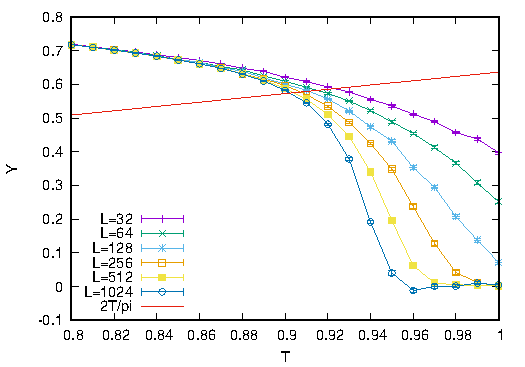
\includegraphics[width=\linewidth]{hm.pdf}
  \caption{正方格子上古典XY 模型のhelicity modulus のモンテカルロ計算。}
  \label{fig:hm}
\end{figure}
\end{document}
